% \documentclass[aspectratio=169,notes]{beamer}
\documentclass[aspectratio=169]{beamer}
\usetheme[faculty=phil]{fibeamer}
\usepackage{polyglossia}
\setmainlanguage{english} %% main locale instead of `english`, you
%% can typeset the presentation in either Czech or Slovak,
%% respectively.
\setotherlanguages{russian} %% The additional keys allow
%%
%%   \begin{otherlanguage}{czech}   ... \end{otherlanguage}
%%   \begin{otherlanguage}{slovak}  ... \end{otherlanguage}
%%
%% These macros specify information about the presentation
\title[Theoretical Mechanics]{Theoretical Mechanics, Lab 11: KIN ENERGY} %% that will be typeset on the
\subtitle{Theorem on the: \\
Change of Kinetic Energy of a System \\ \ } %% title page.
\author{Oleg Bulichev}
%% These additional packages are used within the document:
\usepackage{ragged2e}  % `\justifying` text
\usepackage{booktabs}  % Tables
\usepackage{tabularx}
\usepackage{tikz}      % Diagrams
\usetikzlibrary{calc, shapes, backgrounds}
\usepackage{amsmath, amssymb}
\usepackage{url}       % `\url`s
\usepackage{listings}  % Code listings
% \usepackage{subfigure}
\usepackage{floatrow}
\usepackage{subcaption}
\usepackage{mathtools}
\usepackage{todonotes}
\usepackage{fontspec}
\usepackage{multicol}
\usepackage{pdfpages}
\usepackage{wrapfig}
\usepackage{animate}
\usepackage{booktabs}
\usepackage{multirow}
% \usepackage{graphicx}
\usepackage{colortbl}
\usepackage{catchfilebetweentags}
\usepackage{makecell}
\graphicspath{{resources/}}
\frenchspacing

\setbeamertemplate{caption}[numbered]
\usetikzlibrary{graphs}

% \usepackage[backend=biber,style=ieee,autocite=footnote]{biblatex}
% \addbibresource{biblio.bib}
% \DefineBibliographyStrings{english}{%
%   bibliography = {References},}

\newcommand{\oleg}[2][] {\todo[color=red, #1] {OLEG:\\ #2}}
\newcommand{\fbckg}[1]{\usebackgroundtemplate{\includegraphics[width=\paperwidth]{#1}}}%frame background

\usepackage[framemethod=TikZ]{mdframed}
\newcommand{\dbox}[1]{
\begin{mdframed}[roundcorner=3pt, backgroundcolor=yellow, linewidth=0]
\vspace{1mm}
{#1}
\vspace{1mm}
\end{mdframed}
}

\begin{document}
\setlength{\abovedisplayskip}{0pt}
\setlength{\belowdisplayskip}{0pt}
\setlength{\abovedisplayshortskip}{0pt}
\setlength{\belowdisplayshortskip}{0pt}

\fbckg{fibeamer/figs/title_page.png}
\frame[c]{\setcounter{framenumber}{0}
    \usebeamerfont{title}%
    \usebeamercolor[fg]{title}%
    \begin{minipage}[b][6.5\baselineskip][b]{\textwidth}%
        \textcolor{black}{\raggedright\inserttitle}
    \end{minipage}
    % \vskip-1.5\baselineskip

    \usebeamerfont{subtitle}%
    \usebeamercolor[fg]{framesubtitle}%
    \begin{minipage}[b][3\baselineskip][b]{\textwidth}
        \raggedright%
        \insertsubtitle%
    \end{minipage}
    \vskip.25\baselineskip
}
%   \frame[c]{\maketitle}

\fbckg{fibeamer/figs/common.png}


\section*{Theory}
\begin{frame}[t]{Change of Kinetic Energy of a System}
    \framesubtitle{}
    \scriptsize
        \begin{tabular}{>{\centering\arraybackslash} m{0.9cm}|>{\centering\arraybackslash} m{0.7cm}|>{\centering\arraybackslash} m{4.4cm}|>{\centering\arraybackslash} m{2.3cm}|>{\centering\arraybackslash} m{3.8cm} } 
            \toprule
            \toprule
           \textbf{ R. O.} & \textbf{Eqn \#} & \textbf{Equations} & \textbf{Applications} & \textbf{Extra Info} \\ 
            \hline
            \ExecuteMetaData[../../dynamics_methods_overview/dynamics_methods_overview]{sndkinen}
            \bottomrule
            \bottomrule
            \end{tabular}
    \end{frame}

    \begin{frame}[t]{How to calculate work of reaction forces}
    \framesubtitle{}
        \begin{figure}[H]
            \centering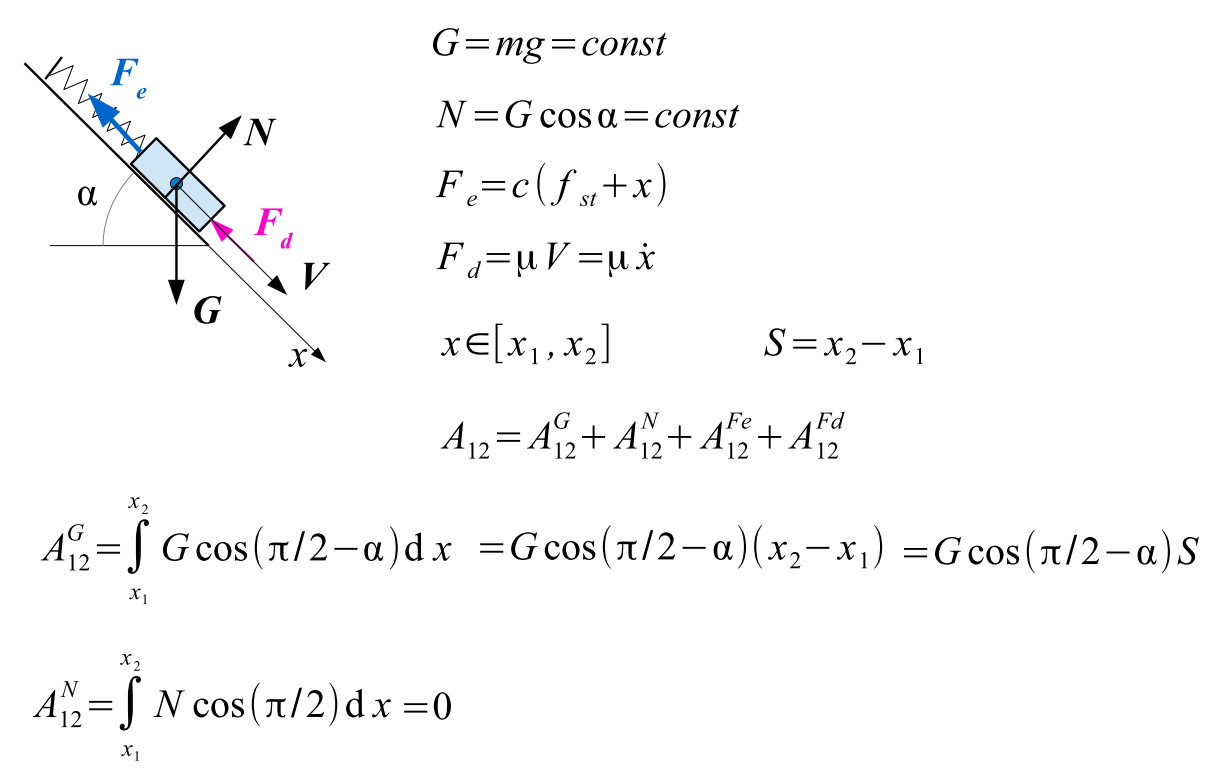
\includegraphics[height=6cm,width=1\textwidth,keepaspectratio]{image7.png}
            \label{fig:image7}
        \end{figure}
    \end{frame}
    
    \begin{frame}[t]{How to calculate work of reaction forces (2)}
    \framesubtitle{}
        \begin{figure}[H]
            \centering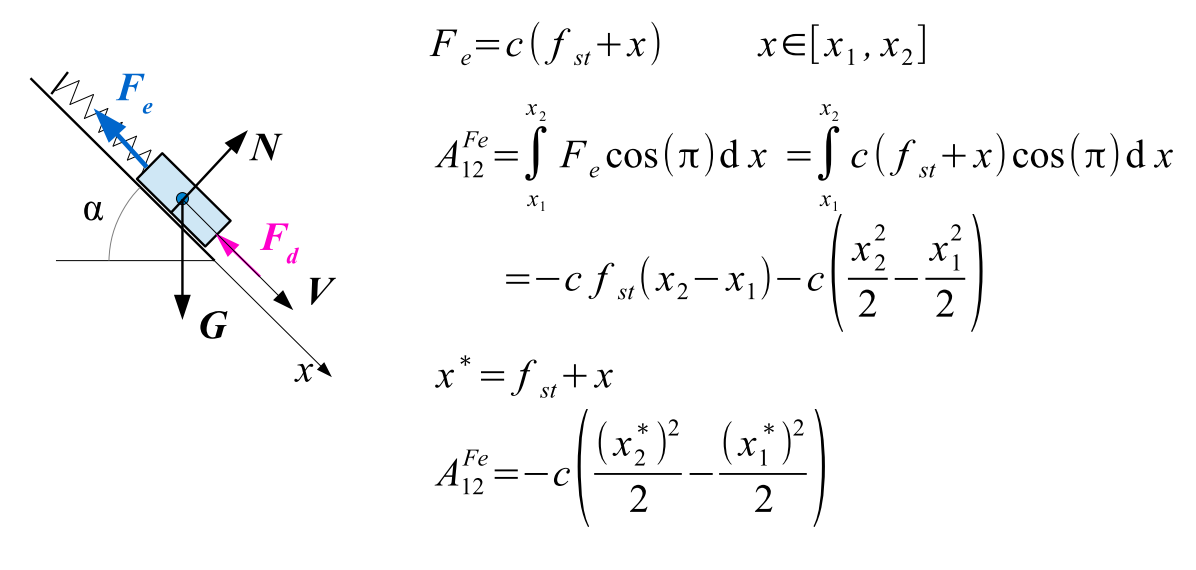
\includegraphics[height=6cm,width=1\textwidth,keepaspectratio]{image12.png}
            \label{fig:image12}
        \end{figure}
    \end{frame}
    
    \begin{frame}[t]{How to calculate work of reaction forces (3)}
    \framesubtitle{}
        \begin{figure}[H]
            \centering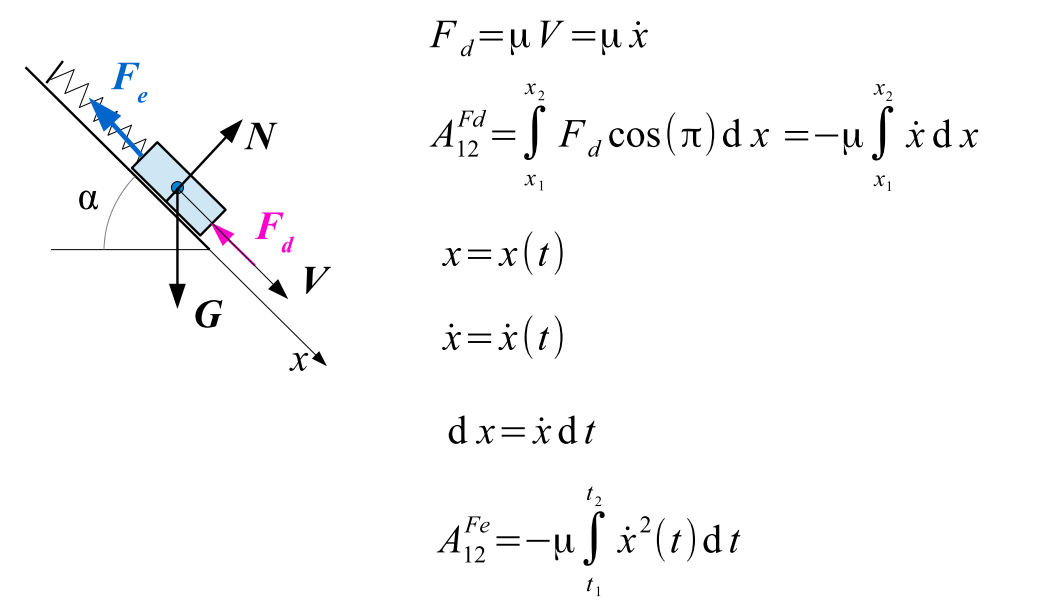
\includegraphics[height=6cm,width=1\textwidth,keepaspectratio]{image14.png}
            \label{fig:image14}
        \end{figure}
    \end{frame}
    
    \begin{frame}[t]{How to calculate work of reaction forces }
    \framesubtitle{}
        \begin{minipage}[H]{0.6\textwidth}
            \textbf{Questions}: Why do we need to find work of N (reaction 
            force) here (when we have slippering) \\
            \textbf{Answer}: Despite that it is internal force, it can have 
            work. 
        \end{minipage}
        \vspace{-0.3cm}
        \begin{figure}[H]
            \flushleft
            \begin{subfigure}[t]{0.59\textwidth}
                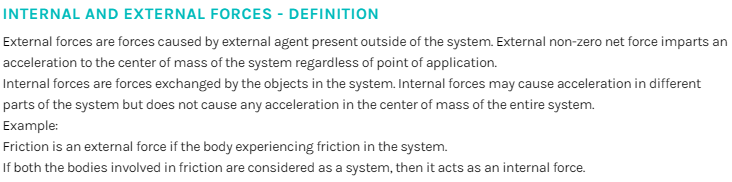
\includegraphics[height=6cm,width=1\textwidth,keepaspectratio]{image21.png}
                \label{fig:image21}
            \end{subfigure}
            \begin{subfigure}[t]{0.39\textwidth}
                \vspace{-3.0cm}
                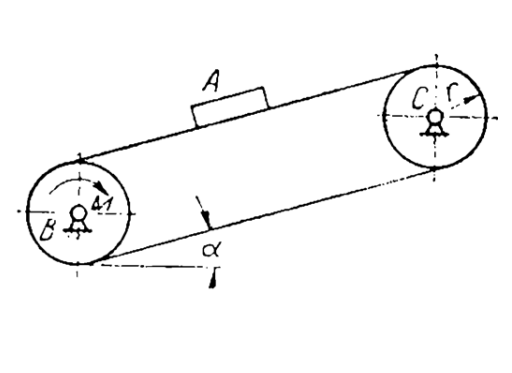
\includegraphics[height=6cm,width=1\textwidth,keepaspectratio]{image2.png}
                \label{fig:image2}
            \end{subfigure}
        \end{figure}
        \begin{minipage}[H]{0.8\textwidth}
            \vspace{-2.5cm}
            \begin{itemize}
                \item We cannot find find work for precise time, only for transfer between two points
                \item $A = F \cdot s$, it is displacement between two bodies who interacts in this force 
                (displacement related from one body to another)
            \end{itemize}
        \end{minipage}
    \end{frame}
    

\section*{Tasks}
\begin{frame}[t]{Task 1 (Mine)}
    \framesubtitle{}
    \small
    A load $A$ of mass $M_1$ has an ideal string attached to it, thrown over the block $D$ of mass $M_2$ and wound on the side surface of the cylindrical roller $B$ of mass $M_3$. 
    \begin{minipage}{0.55\textwidth}

    When load $A$ moves down an inclined plane located at an angle $\alpha$ to the horizon, block $D$ rotates, and the roller $B$ rolls without slippering up the inclined plane, forming an angle $ \beta$.
    \medskip
    
    Determine the velocity $v$ of the load $A$ as a function of its path $s$, if the system is at rest at the initial moment. Consider the block and the roller as homogeneous circular cylinders. The forces of friction are neglected.
    \end{minipage}
    \begin{minipage}{0.44\textwidth}
        \begin{figure}[H]
            \centering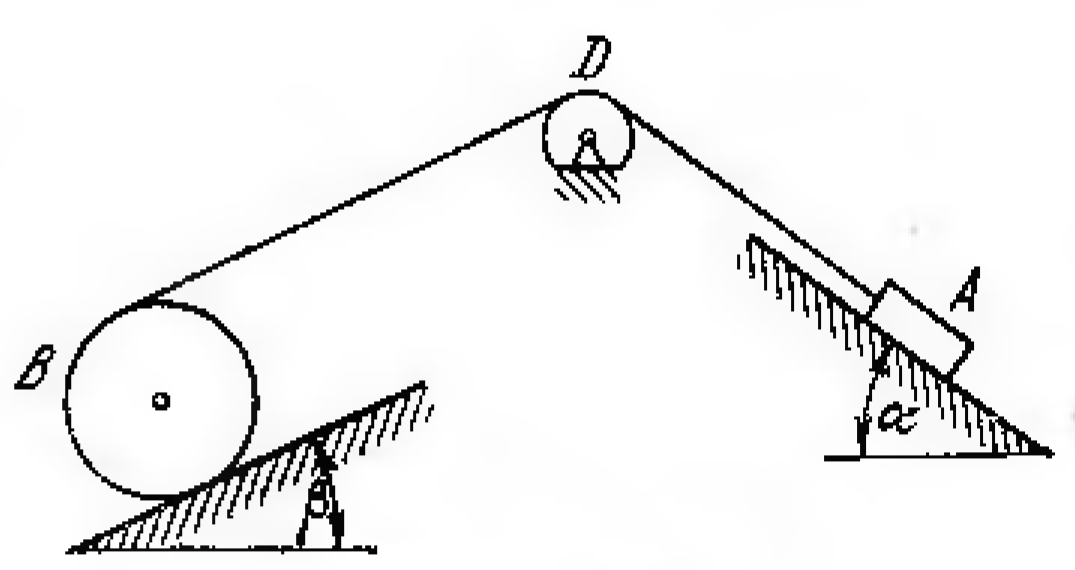
\includegraphics[height=4cm,width=1\textwidth,keepaspectratio]{lab12_1.png}
        \end{figure}
    \end{minipage}
    \end{frame}

    \begin{frame}[t]{Task 2 (yours): M (rus) 38.5}
    \framesubtitle{}
        \begin{figure}[H]
            \begin{subfigure}{0.9\textwidth}
                \centering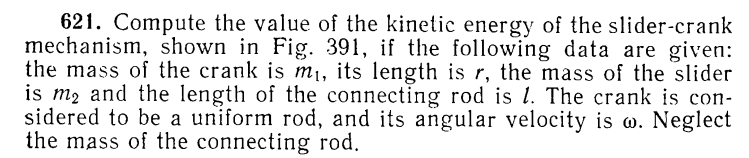
\includegraphics[height=6cm,width=1\textwidth,keepaspectratio]{image11.png}
                % \caption{capture1}
                \label{fig:image11}
            \end{subfigure}
            \begin{subfigure}{0.69\textwidth}
                \centering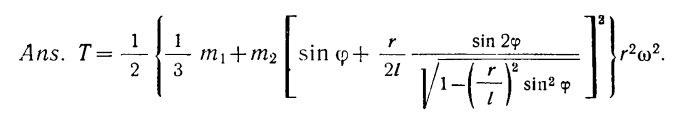
\includegraphics[height=6cm,width=1\textwidth,keepaspectratio]{image13.png}
                % \caption{capture2}
                \label{fig:image13}
            \end{subfigure}
            \begin{subfigure}{0.3\textwidth}
                \vspace{-3.0cm}
                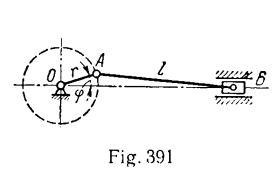
\includegraphics[height=6cm,width=1\textwidth,keepaspectratio]{image15.png}
                % \caption{capture2}
                \label{fig:image15}
            \end{subfigure}
        \end{figure}
    \end{frame}

\begin{frame}[t]{Task 3 (yours): M (rus) 38.20}
\framesubtitle{}
\small
A conveyor belt is set in motion from rest by a drive connected to the lower pulley $B$. The drive imparts a constant torque $M$ to this pulley. The drive gives this pulley a constant torque $M$. 
\begin{columns}[T,onlytextwidth]
    \begin{column}{0.59\textwidth}
Determine the velocity of the conveyor belt $v$ as a function of its displacement $s$, if the mass of the lifted load $A$ is equal to $m_1$, and the pulleys $B$ and $C$ of radius $r$ and mass $m_2$ each are uniform circular cylinders. 
\medskip

The conveyor belt, the mass of which should be neglected, forms an angle $\alpha$ with the horizon. There is no sliding of the belt on the pulleys.
\medskip

\textit{Answer:} $v = \sqrt{\dfrac{2(M-m_1 g r \sin(\alpha))}{r(m_1 + m_2)}s}$

    \end{column}
    \begin{column}{0.39\textwidth}
        \begin{figure}[H]
            \centering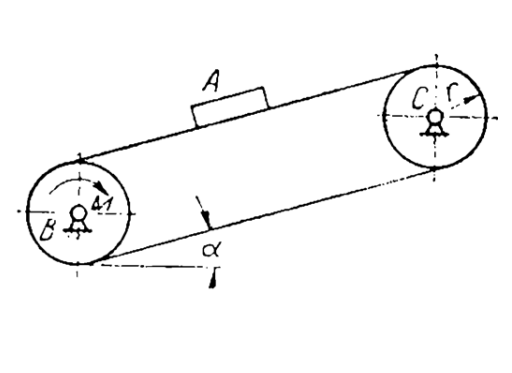
\includegraphics[height=5cm,width=1\textwidth,keepaspectratio]{image2.png}
            % \caption{caption_name}
            \label{fig:image2.png}
        \end{figure}
    \end{column}
\end{columns}
\end{frame}

\begin{frame}[t]{Task 4 (mine)
    }
\framesubtitle{}
\begin{columns}[T,onlytextwidth]
    \begin{column}{0.59\textwidth}
        Find an angular velocity, when the mechanism reaches $-90^\circ$ angle.
        \medskip

        The main goal of the task is to show how to find work in different ways.
    \end{column}
    \begin{column}{0.39\textwidth}
        \vspace{-0.6cm}
        \begin{figure}[H]
            \centering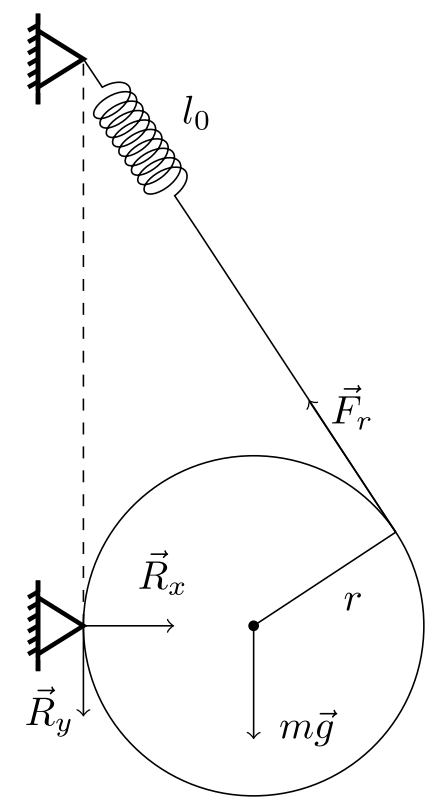
\includegraphics[height=6cm,width=1\textwidth,keepaspectratio]{image16.png}
            \label{fig:image16}
        \end{figure}
    \end{column}
\end{columns}
\end{frame}

\fbckg{fibeamer/figs/last_page.png}
\frame[plain]{}
\end{document}